%%
%%   Version 3.1 of 31 July 2018.
%%
\documentclass[aip,amsmath,amssymb,reprint,floatfix]{revtex4-1}
%\documentclass[aip,reprint]{revtex4-1}

\usepackage{graphicx}% Include figure files
\usepackage{dcolumn}% Align table columns on decimal point
\usepackage{bm}% bold math
%\usepackage[mathlines]{lineno}% Enable numbering of text and display math
%\linenumbers\relax % Commence numbering lines

% hyphenation
\usepackage{hyphenat}

% tables
%\usepackage{dcolumn}
\usepackage{multirow}
%\usepackage{hhline}
\usepackage{booktabs}
%\usepackage{longtable}

% mathematics
\usepackage{amsmath}
\usepackage{amsfonts}
\usepackage{amssymb}
\usepackage{amsbsy}
%\usepackage{bm}
\usepackage{mathrsfs}
\usepackage{upgreek}
%\allowdisplaybreaks

% symbols
%\usepackage{gensymb}
%\usepackage{textcomp}

%---------------------------------------------------
% happy integral
\newcommand{\rint}[1]{\mbox{\Large $ \int\limits_{\mbox{\tiny  $#1$}}$}}
% SHORTCUTS
%\newcolumntype{,}{D{.}{,}{2}}
\newcommand{\citee}[1]{\ensuremath{\scriptsize^{\citenum{#1}}}}
\newcommand{\HRule}{\rule{\linewidth}{0.2mm}}
% Quantum notation
\newcommand{\bra}[1]{\ensuremath{\bigl\langle {#1} \bigl\lvert}}
\newcommand{\ket}[1]{\ensuremath{\bigr\rvert {#1} \bigr\rangle}}
\newcommand{\braket}[2]{\ensuremath{\bigl\langle {#1} \bigl\lvert {#2} \bigr\rangle}}
\newcommand{\tbraket}[3]{\ensuremath{\bigl\langle {#1} \bigl\lvert {#2} \bigl\lvert {#3} \bigr\rangle}}
% Math
\newcommand{\pd}{\ensuremath{\partial}}
\newcommand{\DR}{\ensuremath{{\rm d} {\bf r}}}
%\newcommand{\BM}[1]{\ensuremath{\mbox{\boldmath${#1}$}}}
\newcommand{\BM}[1]{\bm{#1}}
% Chemistry (formulas)
\newcommand{\ch}[2]{\ensuremath{\mathrm{#1}_{#2}}}
% Math 
\newcommand{\VEC}[1]{\ensuremath{\mathrm{\mathbf{#1}}}}
% vector nabla
\newcommand{\Nabla}{\ensuremath{ \BM{\nabla}}}
% derivative
\newcommand{\FDer}[3]{\ensuremath{
\bigg(
\frac{\partial #1}{\partial #2}
\bigg)_{#3}}}
% diagonal second derivative
\newcommand{\SDer}[3]{\ensuremath{
\biggl(
\frac{\partial^2 #1}{\partial #2^2}
\biggr)_{#3}}}
% off-diagonal second derivative
\newcommand{\SSDer}[4]{\ensuremath{
\biggl(
\frac{\partial^2 #1}{\partial #2 \partial #3}
\biggr)_{#4}}}
% derivatives without bound
% derivative
\newcommand{\fderiv}[2]{\ensuremath{
\frac{\partial #1}{\partial #2}}}
% diagonal second derivative
\newcommand{\sderiv}[2]{\ensuremath{
\frac{\partial^2 #1}{\partial #2^2}
}}
% off-diagonal second derivative
\newcommand{\sderivd}[3]{\ensuremath{
\frac{\partial^2 #1}{\partial #2 \partial #3}
}}
% derivatives for tables
\newcommand{\fderivm}[2]{\ensuremath{
{\partial #1}/{\partial #2}}}
% diagonal second derivative
\newcommand{\sderivm}[2]{\ensuremath{
{\partial^2 #1}/{\partial #2^2}
}}
% off-diagonal second derivative
\newcommand{\sderivdm}[3]{\ensuremath{
{\partial^2 #1}/{\partial #2 \partial #3}
}}
% ERIs and OEIs
\newcommand{\OEIc}[3]{\ensuremath{\left(#1 \lvert #2 \rvert #3 \right)}}
\newcommand{\ERIc}[4]{\ensuremath{\left(#1 #2 \vert #3 #4 \right)}}

% Partial density and potential
\newcommand{\PartPot}[4]{\ensuremath{\frac{#1 #2}{\lvert #3-#4 \rvert }}}

% trace operator
\DeclareMathOperator{\Tr}{Tr}

%\draft % marks overfull lines with a black rule on the right

\begin{document}

\preprint{AIP/123-DMS}

\title{One-Particle Density Matrix Polarization Susceptibility Tensors}

\author{Bartosz B{\l}asiak}
\email[]{blasiak.bartosz@gmail.com}
\homepage[]{https://www.polonez.pwr.edu.pl}
%\thanks{Bulak}
\affiliation{Department of Physical and Quantum Chemistry, Faculty of Chemistry, 
Wroc{\l}aw University of Science and Technology, 
Wybrze{\.z}e Wyspia{\'n}kiego 27, Wroc{\l}aw 50-370, Poland}

\date{\today}

\begin{abstract}

%Considering the solvent effect on the correlated electronic wavefunctions, especially
%those that describe the electronically excited state, is a great challenge of Quantum Chemistry. 

The electric field\hyp{}induced change in the one\hyp{}electron density
has been expressed as a series of the one\hyp{}particle density matrix 
susceptibilities (DMS) interacting with the spatial distribution of electric field.
The analytical approximate expressions are derived at the Hartree\hyp{}Fock theory, 
which serves as a basis for construction of generalized model 
that can be used for an arbitrary form of wavefunction as long as the one\hyp{}particle
density matrices are available. It is shown that it is possible to accurately predict 
the changes in the one\hyp{}electron ground\hyp{}state density of water molecule 
in spatially uniform electric field, as well as in spatially non\hyp{}uniform 
electric field distribution generated by point charges. When both linear 
and quadratic terms with respect to the electric field are accounted for,
the electric field\hyp{}induced polarization energies, dipole moments 
and quadrupole moments are quantitatively described by the present theory 
in electric fields from weak to very strong in magnitude (0.003 -- 0.07 a.u.).
It is believed that the proposed model could open new routes in Quantum Chemistry 
for fast and efficient calculations of molecular properties in condensed phases.
\end{abstract}

\pacs{}% insert suggested PACS numbers in braces on next line

\maketitle %\maketitle must follow title, authors, abstract and \pacs

\section{\label{s:1}Introduction}

Molecular\hyp{}level exploration of condensed phase phenomena becomes increasingly unavoidable
as technology and medicine continue to develop. Unfortunately, the computational cost of accurate
electronic structure calculations grows extremely fast with the number of particles, greatly limiting
the use of the state\hyp{}of\hyp{}the\hyp{}art first\hyp{}principles theories 
when large and complex chemical systems such as
solutions and biomolecules come into play.\cite{Tomasi.Mennucci.Cammi.ChemRev.2005}
Due to this reason, it has been of particular importance nowadays 
to develop bridging theoretical techniques that link
extremely accurate but localized pieces of information 
with certain knowledge of an atomistic organisation and intermolecular interaction
on a relatively large spatial scales, typically ranging beyond few nanometers. 

The development of hybrid methods such as quantum mechanical\hyp{}molecular mechanical (QM/MM)
technique was a revolution in computational chemistry which allows insightful theoretical studies
of quantum mechanical effects in biological systems because the costly quantum mechanical calculations
could be combined with lower\hyp{}level and much less expensive
classical dynamics.\cite{Warshel.Levitt.JMolBiol.1976,Senn.Thiel.Angew.2009}
Understanding physics that rules intermolecular interactions\cite{Jeziorski.Moszynski.Szalewicz.ChemRev.1994} 
helped to develop
a wide family of force fields, and served as a basis for embedding Hamiltonian
within an effective environment and fragmentation methods.\cite{Gordon.Fedorov.Pruitt.Slipchenko.ChemRev.2012}

However, even with the modern advances in computational chemistry, 
accurate description of phenomena due to complex heterogeneous molecular environments 
remains a challenge in the following areas: (i) describing the electronically excited states 
(electronic solvatochromism),\cite{Barbati.JACS.2014,
Szabla.Sponer.Jiri.Gora.JPCL.2015,
Bednarska.Zalesny.Tian.Murugan.Agren.Bartkowiak.Molecules.2017,
Jedrzejewska.Grabarz.Bartkowiak.Osmialowski.SpectChimActA.2018} 
(ii) understanding the vibrational properties of molecules in ground and electronically excited states
(vibrational or vibronic solvatochromisms).\cite{Blasiak.Londergan.Webb.Cho.ACR.2017} 
Interface between QM and MM levels is usually realized by electrostatic embedding
and only rarely the Pauli exclusion principle and dispersion are additionally included.\cite{List.Olsen.Kongsted.PCCP.2016}
Unfortunately, it is quite difficult to efficiently treat the environment\hyp{}induced potential operator
due to the complicated nature of intermolecular interactions that theoretically
cannot be solely envisioned as a sum of electrostatic, dispersion and Pauli effects.
One of the most frequently used, efficient and reasonably accurate \emph{ab initio} fragmentation methods,
the effective fragment potential (EFP) methods, are limited to the ground\hyp{}state
chemistry at the Hartree\hyp{}Fock (HF)\cite{Roothaan.RevModPhys.1951,Gordon.Smith.Xu.Slipchenko.AnnuRevPhysChem.2013} 
or density functional theory (DFT) levels\cite{Nguyen.Pachter.Day.JCP.2014}.
Unfortunately, while they can approximately describe the environment composed of molecules in their ground states,
they cannot be used for highly correlated wavefunctions such as electronically excited states.

Most of the efforts to theoretically treat extended molecular aggregates are rooted in 
energy\hyp{} (or force field\hyp{})based philosophy. However,
in the past decade there has been considerable interest in density\hyp{}based approaches
of a wider scope and aims.\cite{Piquemal.Cisneros.Reinhardt.Gresh.Darden.JCP.2006,
Mandado.Hermida-Ramon.JCTC.2011,
Sun.Chan.ACR.2016,
Hedegard.Reiher.JCTC.2016} 
In particular, the importance of
one\hyp{}electron densities in chemistry is well known and acknowledged in the community,\cite{Holas.March.PhysRevA.1991}
though obtaining the exact density has been an undersolved issue for most of chemical systems.
Given that fact, it would be incredibly insightful 
to establish a first\hyp{}principles connection between the one\hyp{}particle
density and the perturbation in the environment through introduction of
\emph{density matrix susceptibility} (DMS) tensors. 
The main postulate of the present work is that the associated change 
in the one\hyp{}particle density matrix, $\delta {\bf D}$, can be
represented in a product form of the generalized perturbation susceptibility ${\bf B}_i$
and the environment\hyp{}induced perturbation on a molecule, $\delta {\bf P}_i$,
evaluated at certain site $i$.
%
\begin{equation*} \label{e:initial-model}
  \delta {\bf D} \approx \sum_i^{\text{Sites}} {\bf B}_i
  \cdot  \delta {\bf P}_i \;.
\end{equation*}
%
While $\delta {\bf P}_i$ contains critical information 
about the actual distortion of the electronic cloud,
perturbation susceptibility is assumed to be a property of unperturbed 
molecule and is to be precomputed only once. 
Thus, such DMS could be adapted into an efficient effective 
one\hyp{}electron fragment potential which in principle, is applicable to an arbitrary
level of theory, as long as the one\hyp{}particle densities are available.
It also means that such a technique would dramatically reduce costs of quantum chemistry calculations
because the task of performing full computation on a molecular aggregate
would reduce to much simpler matrix operations.

The simplest type of perturbation, yet the most relevant for chemistry, 
is the electrostatic perturbation.
It is worth mentioning that, at the moment, there is no simple \emph{ab initio}
method to compute electron deformation densities without considering the entire molecular 
aggregate by using full quantum chemistry calculations.\cite{Horn.Head-Gordon.JCP.2015,
Mandado.Hermida-Ramon.JCTC.2011}
In this work, we explore the susceptibility of the molecule's electronic density distribution
to polarize due to external electrostatic perturbation from first principles. 
The deformation density is expressed in terms
of the one\hyp{}particle density matrix polarization susceptibility tensors 
that are properties of isolated molecules and can be
extracted from quantum chemistry calculations. The focus on the density (matrix) instead of the energy
(scalar) is beneficial since it provides the directional tensor description
of the polarization that could be combined with other effects such as Pauli repulsion 
or dispersion,\cite{Mandado.Hermida-Ramon.JCTC.2011}
in contrast to the standard interaction energy approaches. We show that accurate polarization 
of the one\hyp{}particle density
matrix is achievable and can be realized as long as the one\hyp{}particle density matrices
are available. It is believed that the proposed method
could be a basis for a construction of an 
alternative approach in fragment\hyp{}based
modelling of extended molecular aggregates that is not limitted to the ground state chemistry.

We introduce the necessary theory and derive the \emph{ab initio} density matrix susceptibility model
at the HF approximation\cite{Roothaan.RevModPhys.1951} 
in Section~\ref{s:2}. Subsequently, this model serves as a basis for generalization to the 
arbitrary one\hyp{}electron density with electronic correlation which is derived in Section~\ref{s:2}. 
The implementation details in a computer code as well as the validation procedures are detailed
in Section~\ref{s:3}. We then discuss the performance of the models in Section~\ref{s:4}.
Finally, in Section~\ref{s:5} we conclude the presentation with a few 
remarks for future development.

\section{\label{s:2}Theory}

The electronic energy of a closed\hyp{}shell molecule is given by the time\hyp{}independent Schr{\"o}dinger equation,
%
\begin{equation}
 E^{(0)} = \tbraket{\Psi^{(0)}}{\mathscr{H}^{(0)}}{\Psi^{(0)}} \;,
\end{equation}
%
where $E$ stands for the total electronic energy, $\Psi$ the electronic wavefunction and $\mathscr{H}$
the Hamiltonian operator. In the above, the superscript $(0)$
denotes the reference or unperturbed state that is assumed to be known.
Under the influence of an external electrostatic perturbation, the total electronic energy
becomes
%
\begin{equation}
 E[{\bf F}({\bf r})] = \tbraket{\Psi}{\mathscr{H}^{(0)} + \mathscr{V}({\bf F}({\bf r}))}{\Psi}
\end{equation}
%
in which ${\bf F}({\bf r})$ is a non\hyp{}uniform electric field distribution.
The electric field\hyp{}induced energy change is an unknown functional 
of the associated change in the one\hyp{}electron density,
%
\begin{equation}\label{e:rho}
 \rho({\bf r}) = 2\sum_{\alpha\beta} D_{\alpha\beta} \phi_\alpha({\bf r}) \phi^*_\beta({\bf r}) \;.
\end{equation}
%
In Eq.~\eqref{e:rho} $\phi_\alpha({\bf r})$ is a basis funtion, which can be for instance 
an atomic orbital (AO) or a molecular orbital (MO), and $D_{\alpha\beta}$ is the corresponding
one\hyp{}particle density matrix.
If perturbation\hyp{}independent basis is chosen, the electric field\hyp{}induced change in the one\hyp{}particle density
is given by
%
\begin{equation}\label{e:rho-1}
 \delta \rho({\bf r}) = 2\sum_{\alpha\beta} \delta D_{\alpha\beta} \phi_\alpha({\bf r}) \phi^*_\beta({\bf r}) \;.
\end{equation}
%
The electric field\hyp{}induced change in the ground state's one\hyp{}particle density 
follows its energy minimum of the perturbed state. In addition, all the perturbed 
excited state one\hyp{}electron densities must be excited state solutions of the Schr{\"o}dinger equation
with the exact energy\hyp{}minimized ground state. 

In the limit of a weak and spatially uniform electric field,
the polarization\hyp{}induced density matrix change is given by the following Taylor expansion:
%
\begin{equation}\label{e:dD-Taylor}
 \delta D_{\alpha\beta} = \frac{\partial D_{\alpha\beta}}{\partial {\bf F}}\Bigg|_{{\bf F}={\bf 0}}  \cdot {\bf F} 
   + \frac{1}{2} 
     \frac{\partial^2 D_{\alpha\beta}}{\partial {\bf F} \otimes \partial {\bf F}}\Bigg|_{{\bf F}={\bf 0}} : {\bf F} \otimes {\bf F}
   + \ldots 
\end{equation}
%
In the above expression, the density matrix susceptibilities are simply equal to the derivatives of the density matrix
with respect to electric field (up to a multiplicative constant).
In a general case, i.e., when electric field is non\hyp{}uniform, the development of a first\hyp{}principles theory
that is capable of accurately capturing the electric field\hyp{}dependence of the one\hyp{}particle density
becomes extremely difficult. This is not only because of the very complicated (and generally unknown) solution
to the electronic correlation problem, but also because
a working model has to accurately predict all the $n^2$ elements of the density matrix
where $n$ is the size of basis set. Even relatively small errors
in a particular matrix element will accumulate when performing two\hyp{}
and four\hyp{}index contractions,
and in turn, affect the evaluated properties with non\hyp{}negligible errors.
Single\hyp{}centered expansions, like the one from Eq.~\eqref{e:dD-Taylor}, although valid for 
an arbitrary level of theory,
are not sufficient enough to accurately describe the local polarization
of electron density distribution when electric fields are highly non\hyp{}uniform in space.
Due to all of these reasons, we adopt the following approach: 
we first develop a qualitative first\hyp{}principles distributed\hyp{}site model at the Hartree\hyp{}Fock
level of theory, and then generalize it to the arbitrary level using the functional form that was found 
by considering HF level,
but treating the density matrix susceptibility tensors as cetrain functions of adjustable parameters further on.

\subsection{Ab Initio Density Matrix Susceptibilities: Hartree-Fock Level}

\subsubsection{Induced Dipole Moment}

$\delta {\bf D}$ should 
be directly related to the
polarization\hyp{}induced multipole moments because they are
a measure of the distortion of the electron density distribution due to the external electric
field. 
Therefore, 
we start our analysis by considering the induced electronic dipole moment 
of a closed-shell molecule, 
%
\begin{equation} \label{e:dmu-exact}
 \delta {\BM{\upmu}}({\bf r}_Q) = 
     2 \Tr{ 
         \left[ 
              \delta {\bf D} \cdot {\mathbb{M}({\bf r}_Q)}
         \right] } \;,
\end{equation}
%
where ${\mathbb{M}({\bf r}_Q)}$ is atomic orbital (AO)\hyp{}representation
of the dipole moment operator defined with respect to origin at ${\bf r}_Q$,
%
\begin{equation}\label{e:m}
 \left[ {\mathbb{M}({\bf r}_Q)} \right]_{\alpha\beta} = -e\tbraket{\alpha}{{\bf r} - {\bf r}_Q}{\beta} \;.
\end{equation}
%
(In this work we shall use the special open bold font for matrices of vectors, so that
in this case ${\mathbb{M}}$ can be considered as a $n \times n$ matrix of vectors of length 3).
Note that if the total charge is conserved, the induced moments are independent of the origin.

In the Hartree\hyp{}Fock theory,\cite{Roothaan.RevModPhys.1951} ${\bf D}$ is approximated as
%
\begin{equation}
 {\bf D} = {\bf C} \cdot {\bf C}^\dagger \;,
\end{equation}
%
where ${\bf C}$ describes the occupied molecular orbitals (MO's) as linear combinations
of AO's, referred here to as the LCAO-MO matrix.
${\bf D}$ is an idempotent matrix and if expressed in orthogonal basis the following holds
%
\begin{equation}
 {\bf D}^2 = {\bf D} \;.
\end{equation}
%
The change in the molecular orbitals can be parameterized as suggested by McWeeny\cite{McWeeny.RevModPhys.1960}
by defining the idempotency\hyp{}preserving variation
%
\begin{equation}
 \delta {\bf C} = {\BM\Delta} \cdot {\bf C}^{(0)} \;,
\end{equation}
%
where $\BM\Delta$ is a square non\hyp{}singular and non\hyp{}symmetric matrix.
McWeeny showed that
%
\begin{equation} \label{e:dmat-change.exact}
 \delta {\bf D} = -{\bf D}^{(0)} + \left[ {\bf D}^{(0)} + {\bf v} \right] \cdot
                                   \left[ {\bf 1} + {\bf v}^\dagger \cdot {\bf v} \right]^{-1} \cdot
                                   \left[ {\bf D}^{(0)} + {\bf v}^\dagger \right] \;,
\end{equation}
%
where the auxiliary vector ${\bf v}$ is defined as
%
\begin{equation}
 {\bf v} \equiv \left[ {\bf 1} - {\bf D}^{(0)} \right] \cdot {\BM\Delta} \cdot {\bf D}^{(0)}  \;.
\end{equation}
%
Expanding Eq.~\eqref{e:dmat-change.exact} in a Taylor series around ${\bf v}={\bf 0}$ and
truncating it at linear terms with respect to ${\BM\Delta}$ gives
%
\begin{subequations} 
 \begin{align}
 \delta {\bf D} &\cong \left[ {\bf 1} - {\bf D}^{(0)} \right] \cdot {\BM\Delta} \cdot {\bf D}^{(0)} + 
                        {\bf D}^{(0)} \cdot {\BM\Delta}^\dagger \cdot \left[ {\bf 1} - {\bf D}^{(0)} \right]  
 \label{e:dD-1} \\  &= 
  \delta {\bf C} \cdot {\bf C}^{(0)\dagger} + {\bf C}^{(0)} \cdot \delta {\bf C}^\dagger \nonumber \\
           &\qquad - {\bf D}^{(0)} \cdot \delta {\bf C} \cdot {\bf C}^{{(0)}\dagger} 
                   - {\bf C}^{(0)} \cdot \delta {\bf C}^\dagger \cdot {\bf D}^{(0)}  \;.
 \label{e:dD-2}
 \end{align}
\end{subequations}
%
The latter equality is true only if the basis set functions are orthogonal, i.e., 
${\bf C}^{(0)\dagger} \cdot {\bf C}^{(0)}={\bf 1}$,
which will be the case throughout the entire work, unless stated otherwise.
Substituting the result from Eq.~\eqref{e:dD-1}
into Eq.~\eqref{e:dmu-exact} leads to
%
\begin{multline} \label{e:dmu-4-exact.linear-approximation}
 \frac{1}{2} 
 \delta {\BM{\upmu}}
  \cong
   \Tr{ 
    \left[ 
         {\mathbb{M}} \cdot {\BM\Delta} \cdot {\bf D}^{(0)}  
    \right] }
%
  +\Tr{ 
    \left[ 
         {\mathbb{M}} \cdot {\bf D}^{(0)} \cdot {\BM\Delta}^{\dagger}
    \right] } \\
%
  -\Tr{ 
    \left[ 
         {\mathbb{M}} \cdot {\bf D}^{(0)} \cdot {\BM\Delta} \cdot {\bf D}^{(0)}
    \right] }
%
  -\Tr{ 
    \left[ 
         {\mathbb{M}} \cdot {\bf D}^{(0)} \cdot {\BM\Delta}^{\dagger} \cdot {\bf D}^{(0)}
    \right] } \;.
\end{multline}
%
It can be proven (see Appendix~\ref{a:orig-dep}) that such obtained
induced dipole moment is independent of the origin. 
This guarantees that the theory fulfills the total charge conservation requirement.
Therefore,
in the above result and also in later course of the paper the dipole origin will be omitted. 
%where the dipole origin was omitted for notational clarity.

Now, if the AO basis is orthogonal, Eq.~\eqref{e:dmu-4-exact.linear-approximation} can be simplified by realising that
%
\begin{equation}
 \frac{1}{2} 
 \delta {\BM{\upmu}}
  \cong
2 \Tr{ 
    \left[ 
         \widetilde{\mathbb{M}} \cdot \delta {\bf C}
   \right] }  
-
2 \Tr{ 
    \left[ 
         \widetilde{\mathbb{K}} \cdot \delta {\bf C}
   \right] } \;.
\end{equation}
%
Here we introduced the auxiliary tensors
%
\begin{subequations}
 \begin{align}
   \widetilde{\mathbb{M}}  &\equiv {\bf C}^{(0)\dagger} \cdot {\mathbb{M}}     \;,           \\
   \widetilde{\mathbb{K}}  &\equiv {\bf C}^{(0)\dagger} \cdot {\mathbb{M}} \cdot {\bf D}^{(0)} \;, \\
   \widetilde{\mathbb{L}}  &\equiv \widetilde{\mathbb{M}} - \widetilde{\mathbb{K}} \;
 \end{align}
\end{subequations}
%
to simplify the notation. Hence, we have
%
\begin{equation} \label{e:dmu-l-vector}
  \frac{1}{4} 
 \delta {\BM{\upmu}} %({\bf r}_0) 
   =
   \Tr{ 
    \left[ 
         \widetilde{\mathbb{L}} \cdot \delta {\bf C}
    \right] }
   %
   \equiv \sum_{i}^{\rm occ} \sum_\alpha {\bf l}_{i\alpha} \delta C_{\alpha i} \;,
\end{equation}
%
where the Cartesian vector
%
\begin{equation}\label{e:l-vector}
 {\bf l}_{i\alpha} \equiv \left[ \widetilde{\mathbb{M}} - \widetilde{\mathbb{K}} \right]_{i\alpha} 
      = \left[  {\bf C}^\dagger \cdot \mathbb{M} \cdot \left( {\bf 1} - {\bf D}^{(0)} \right) \right]_{i\alpha}
\end{equation}
%
and $i$ runs over occupied unperturbed MO's.
Note that the intermediate quantity $\widetilde{\mathbb{L}}$ contains the projector onto
the unoccupied MO space at the absence of the external electric field. It means that the
perturbed solution is constructed from the unperturbed virtual orbitals as well.
Although Eq.~\eqref{e:dmu-l-vector}
is exact up to first order in ${\BM\Delta}$, it cannot be inverted at this moment to obtain $\delta {\bf C}$
due to the presence of trace operation, unless the electric field is uniform.
Let the induced dipole moment be partitioned into separate contributions
from the occupied MO's, i.e.,
%
\begin{equation} \label{e:dmu-part}
 \delta {\BM{\upmu}} = \sum_i^{\rm occ} \delta {\BM{\upmu}}_i \;,
\end{equation}
%
where
%
\begin{equation} \label{e:dmu-dpol}
 \delta {\BM{\upmu}}_i = {\BM{\alpha}}_i \cdot {\bf F}({\bf r}_i) \;.
\end{equation}
%
In Eq.~\eqref{e:dmu-dpol}, ${\BM{\alpha}}_i$ is the distributed dipole\hyp{}dipole polarizability tensor
associated with the $i$th MO whereas ${\bf F}({\bf r}_i)$ is the electric field evaluated at the $i$th MO centroid of charge,
${\bf r}_i = \tbraket{\phi_i}{\hat{\bf r}}{\phi_i}$.
By inserting the above result into Eq.~\eqref{e:dmu-l-vector},
recasting the right hand side in a matrix form
and assuming real quantities,
one can separate the contributions coming from occupied MO's as
%
\begin{equation} \label{e:dmu-l-vector-mo-transform-X}
 \frac{1}{4} {\BM{\alpha}}_i \cdot {\bf F}({\bf r}_i) 
   =
   \delta {\bf c}_i^T \cdot {\bf L}_i \;.
\end{equation}
%
Note that now ${\bf L}_i$ is a matrix of dimension $n \times 3$ and $\delta{\bf c}_i$ is the $i$th column of the
change in the LCAO-MO matrix due to the polarization process.
The solution for $\delta {\bf C}$ is
%
\begin{equation} \label{e:mu-ind.matrix.linear.solution}
  \delta {\bf c}_i^T = \frac{1}{4}
            {\bf F}({\bf r}_i)  \cdot {\BM{\alpha}}_i \cdot 
                    \left[ {\bf L}_i  \right]^{-1}_{\rm Left} \;,
\end{equation}
%
where $\left[ {\bf L}_i  \right]^{-1}_{\rm Left}$ is a left inverse
of ${\bf L}_i$ matrix,
%
\begin{equation} 
      \left[ {\bf L}_i  \right]^{-1}_{\rm Left}   \equiv
       \left[ {\bf L}_i^T \cdot {\bf L}_i \right]^{-1} \cdot {\bf L}_i^T   
\end{equation}
%
with the dimension of $3\times n$. Note that the right inverse of ${\bf L}_i$
does not exist because ${\bf L}_i \cdot {\bf L}_i^T$ is singular due to the fact that usually
$n > 3$.

\subsubsection{Density Matrix Change}

Now we can obtain the final expression for the density matrix change 
due to external electric field that reproduces the 
induced dipole moment of the molecule.
The change in the LCAO\hyp{}MO coefficient is parameterized as
%
\begin{equation} \label{e:dC-dmatpol}
 \delta C_{\alpha i} = {\bf b}_{\alpha}^{(i;1)} \cdot {\bf F}({\bf r}_i)  \;,
\end{equation}
%
where the susceptibility tensor is defined as
%
\begin{equation} \label{e:susceptibility-b}
  b_{\alpha;w}^{(i;1)}= \frac{1}{4} \sum_u^{x, y, z} \left[ {\BM{\alpha}}_i \right]_{uw}
   \left[ \left[ {\bf L}_i  \right]^{-1}_{\rm Left} \right]_{u;\alpha}  
\end{equation}
%
for $w=x,y,z$. 
The superscript `$(1)$' underlines the fact that the susceptibility introduced here
is first\hyp{}order with respect to the electric field.
The result from Eq.~\eqref{e:dC-dmatpol} can be now inserted into 
the expression for $\delta {\bf D}$ from Eq.~\eqref{e:dD-2} to finally give
%
\begin{equation}\label{e:final-model.HF}
 \delta D_{\alpha\beta} \approx \sum_i^{\rm occ} {\bf B}^{(i;1)}_{\alpha\beta} \cdot {\bf F}({\bf r}_i)  \;,
\end{equation}
%
where the \emph{density matrix polarization susceptibility tensor} is
%
\begin{multline}  \label{e:susceptibility-B}
 {\bf B}^{(i;1)}_{\alpha\beta} = 
                               C_{\alpha i} {\bf b}_{\beta}^{(i;1)} + C_{\beta i} {\bf b}_\alpha^{(i;1)} \\
                                - \sum_\gamma 
                                 \left( 
               D_{\alpha\gamma} C_{\beta i} + D_{\beta\gamma} C_{\alpha i}
                                 \right)
                                           {\bf b}_{\gamma}^{(i;1)}
 \;.
\end{multline}
%
Hence, the three dimensional vector ${\bf B}^{(i;1)}_{\alpha\beta}$ describes the polarization affinity
of the density matrix element associated with the $\alpha$th and $\beta$th orthogonal AO's.
Transforming these vectors to a non\hyp{}orthogonal AO basis is straightforward.
It is emphasized here that all elements of ${\bf B}_{\alpha\beta}^{(i;1)}$
are unique properties of electronically unperturbed molecule. 

One very important feature of the susceptibility from Eq.~\eqref{e:final-model.HF} is that
the density matrix increment is dependent \emph{only} on the susceptibility element associated with the same
pair of AO's. Therefore, there is no mixing in the AO's, rather the increment is proportional to the 
vector susceptibility, different for each density matrix element. This feature will be used to
generalize the model to an arbitrary level of theory and electric field curvature in the next section.

\subsection{Generalized Density Matrix Susceptibility Model}

\subsubsection{Functional form of the model}

Eq.~\eqref{e:final-model.HF}, which is the final result of the previous section, 
can be used as a guideline to construct a general model of density matrix polarization.
Quadratic (and higher\hyp{}order) terms with respect to the electric field
can be added to the formulation, which leads to
%
\begin{multline}\label{e:final-model.General}
 \delta D_{\alpha\beta} = \sum_{i }^M \Big\{
                                      {\bf B}^{(i ; 1)}_{\alpha\beta} \cdot {\bf F}({\bf r}_i)  \\
%                       + \sum_{ij}^M {\bf B}^{(ij; 2)}_{\alpha\beta} : {\bf F}({\bf r}_i) \otimes {\bf F}({\bf r}_j)
                        +             {\bf B}^{(i ; 2)}_{\alpha\beta} : {\bf F}({\bf r}_i) \otimes {\bf F}({\bf r}_i) 
                        + \ldots \Big\} \;.
\end{multline}
%
In the above equation, the density matrix susceptibilities
${\bf B}^{(i; R)}_{\alpha\beta}$, distributed over $M$ sites,
denote the $R$-th order response with respect to the electric field.
Note that
${\bf B}^{(i; 1)}_{\alpha\beta}$ is a vector of length $3$ whereas ${\bf B}^{(i; 2)}_{\alpha\beta}$
is a $3\times 3$ matrix. Also, the distributed expansion centres
(labeled as $i$) are generalized to any point in the molecule.\footnote{More general
contribution due to square of electric field could 
be $\sum_{ij}^M {\bf B}^{(ij; 2)}_{\alpha\beta} : {\bf F}({\bf r}_i) \otimes {\bf F}({\bf r}_j)$. 
However, for simplicity, we neglect the contributions from different sites $i$ and $j$
in the present discussion and leave it for future development.
}

\subsubsection{Determining the generalized susceptibility tensors}

The exact mathematical form of the generalized density matrix susceptibilities 
from Eq.~\eqref{e:final-model.General} is unknown. 
The susceptibility from Eq.~\eqref{e:final-model.HF} is valid only under the Hartree\hyp{}Fock
approximation, with a guarantee that only the overall charge (exactly) and the dipole moment (approximately,
limited by the flavour of the distributed polarizability approximation), 
but not higher multipole moments and polarization energy, are correctly described.
Our strategy is to treat the susceptibilities from Eq.~\eqref{e:final-model.General}
as adjustable parameters, rather than try to derive them from the first principles theory.

Let  
$\left\{ {\bf F}^{(1)}({\bf r}), {\bf F}^{(2)}({\bf r}), \ldots, {\bf F}^{(N)}({\bf r}), \ldots \right\}$ 
be a set of $N_{\rm max}$ distinct and randomly sampled 
spatial distributions of electric field. It is assumed that
the exact difference one\hyp{}particle density matrices (with respect to the unperturbed state)
defined as
%
\begin{equation}
 \delta \overline{\bf D}^{(N)} \equiv \overline{\bf D}^{(N)} - \overline{\bf D}^{(0)}
\end{equation}
%
are known for each sample (overline symbolizes the exact estimate).
Now, for each pair of the AO indices we construct the following 
parameterization of Eq.~\eqref{e:final-model.General}:
%
\begin{multline}\label{e:final-model.General.Parameters}
 \delta D^{(N)} = \sum_{i }^M \Big\{ 
                              \sum_u^{x,y,z} S^{[1]}_{iu} F_{iu}^{(N)} \\
%               + \sum_{ij}^M \sum_{uw}^{x,y,z} \left( S^{[2]}_{iu} + S^{[2]}_{jw} \right) F_{iu}^{(N)} F_{jw}^{(N)}
                +             \sum_{u}^{x,y,z} \sum_{w<u} r_{uw} S^{[2]}_{iuw} F_{iu}^{(N)} F_{iw}^{(N)} 
                        + \ldots \Big\}
\end{multline}
%
(the Greek subscripts were omitted here for notational simplicity).
In the above equation, $B_u^{(i;1)} = S^{[1]}_{iu}$ and $B_{uw}^{(i;2)} = r_{uw} S^{[2]}_{iuw}$,
where $r_{uw}$ is the symmetry factor equal to 1 for diagonal elements and 2 for off\hyp{}diagonal
elements of $B_{uw}^{(i;2)}$.
Note that the multiple parameter blocks 
${\bf S}^{[1]}$ and ${\bf S}^{[2]}$
appear in the first power, allowing for linear least\hyp{}squares regression.
The square bracket superscripts denote the block of the parameter space. 

To determine the optimum set 
$
 {\bf S} = 
\begin{pmatrix}
{\bf S}^{[1]} &
{\bf S}^{[2]} 
\end{pmatrix}^T
$, we define a loss function $Z$ 
of the two blocks of adjustable parameters
that is subject to the least\hyp{}squares minimization,
%
\begin{equation}\label{e:Z}
 Z[{\bf S}] = \sum_N^{N_{\rm max}} \left( \delta D^{(N)} - \delta \overline{D}^{(N)} \right)^2 \;.
\end{equation}
%
The Hessian of $Z$ computed with respect to the parameters 
is parameter\hyp{}independent (constant) and generally non\hyp{}singular
as long as the electric fields on all distributed sites are different.
Therefore, the exact solution for the optimal parameters is given by the Newton equation
%
\begin{equation}\label{e:Newton}
 {\bf S} = -{\bf H}^{-1} \cdot {\bf g} \;,
\end{equation}
%
where ${\bf g}$ and ${\bf H}$ are the gradient vector and the Hessian matrix, respectively.
The explicit forms of the gradient and Hessian are given in the Appendix~\ref{a:blocks}.
Note that the dimensions of parameter space for the block 1 and 2 are
equal to $3M$ and $6M$, respectively.

\section{\label{s:3}Calculation Details}

The theory that is necessary to validate the density matrix susceptibility models from Section~\ref{s:2}
was implemented in our in\hyp{}house plugin to {\sc Psi4} quantum chemistry program.\cite{Psi4.JCTC.2017}
Water molecule
was selected as a test system which was subjected to 
electrostatic perturbations due to random uniform electric fields and random collections of point charges
generating non\hyp{}uniform electric fields. 
Components of spatially uniform electric fields were determined 
from the uniform distribution in the interval of $\vert 0.0404 \vert$ a.u.
generating average field of 0.035 a.u. in an ensemble of 100 samples.
Cartesian coordinates of point charges were drawn from the uniform distribution 
of a set of fourty three\hyp{}dimensional Euclidean points within a sphere of radius 6.0 Bohrs
with an origin that is located in the center of mass of water molecule.
In selection of random points, space inside the union of spheres surrounding
oxygen and hydrogen atoms with radii of 4.5 and 4.0 Bohrs, respectively, was
kept free from any point charges due to potential problems with the convergence of the 
self\hyp{}consistent field (SCF) calculations.
Electric charge values were selected from the one\hyp{}dimensional uniform distribution
of double precision numbers in the interval of $\vert q_{\rm max} \vert$, where $q_{\rm max}$
was tuned to obtain a desired ensemble of weak, moderate and strong electric field magnitudes
(with $q_{\rm max}=0.05$, $0.2$ and $0.4$ a.u., accordingly).
In this way, independent sets of 100 random samples of uniform electric fields as well as 
40 point charges were selected and exact solutions of HF\hyp{}SCF equations were 
performed for each validation procedure.

In order to validate all the models discussed in this contribution,
the electric field\hyp{}induced polarization energy, 
dipole moment and quadrupole moment were analysed in detail.
The electric field\hyp{}induced polarization energy at the HF level, $\delta E^{\rm Pol}$,
was computed from the following exact formula:
%
\begin{multline}\label{e:dE}
 \delta E^{\rm Pol}[{\bf F}] = 
                     \Tr{\left\{ {\bf D}^{(0)} \cdot
                                \left( 2\delta {\bf J} - \delta {\bf K}  \right) \right\}} \\
                   + \Tr{\left\{ \delta {\bf D} \cdot
                                \left( {\bf H}^{(0)} + {\bf f}^{(0)} + 2{\bf V} + 2\delta {\bf J} - \delta {\bf K}\right) \right\}} \;.
\end{multline}
%
In Eq.~\eqref{e:dE}, ${\bf f}^{(0)}$ and ${\bf H}^{(0)}$ are the Fock matrix and 
the one\hyp{}electron Hamiltonian matrix of an unperturbed HF ground state,
${\bf V}$ is the one\hyp{}electron external electrostatic potential matrix whereas $\delta {\bf J}$
and $\delta {\bf K}$ are electric field\hyp{}induced changes in the Coulomb and the exchange HF matrices due to 
the polarization of the electron density distribution, respectively. 
In order to compare the performance of the usual 
distributed dipole\hyp{}dipole polarizability approach,
the approximate interaction energy was also evaluated by using the expression:
%
\begin{equation}\label{e:dE-dpol}
 \delta E^{\rm Pol}[{\bf F}] \approx 
                   - \frac{1}{2} \sum_i^{\rm occ} {\BM \alpha}_i : {\bf F}({\bf r}_i) \otimes {\bf F}({\bf r}_i) \;,
\end{equation}
%
in which ${\BM \alpha}_i$ is the distributed anisotropic dipole\hyp{}dipole polarizability tensor associated with the
$i$th localized molecular orbital (LMO) centroid (see Eq.~\eqref{e:dmu-dpol}).
The distributed polarizabilities were computed by utilizing the coupled\hyp{}perturbed Hartree\hyp{}Fock
method.\cite{McWeeny.RevModPhys.1960,Dodds.McWeeney.Sadlej.MolPhys.1977} 
Orbital localization was performed by using the Boys method.\cite{Boys.RevModPhys.1960} 

The electric field\hyp{}induced dipole and primitive quadrupole moments were evaluated from the following expressions:
%
\begin{subequations}\label{e:dmult}
  \begin{align}
   \delta \upmu_{u}   &= 2\sum_{\alpha\beta} \delta D_{\alpha\beta} \tbraket{\alpha}{u}{\beta}  \;,\\
   \delta \Theta_{uw} &= 2\sum_{\alpha\beta} \delta D_{\alpha\beta} \tbraket{\alpha}{(u-u_{\rm CM})(w-w_{\rm CM})}{\beta} \;, 
  \end{align}
\end{subequations}
%
where the subscript `CM' denotes the center of mass of water molecule.
When the distributed polarizabilities were used instead of the polarization\hyp{}induced 
difference density matrices, primitive induced quadrupole moments were computed from
the induced dipole moments (given in Eq.~\eqref{e:dmu-dpol}) according to
%
\begin{equation}
  \delta {\BM \Theta} = \sum_i^{\rm occ} 
   \left\{ 
       \delta {\BM \upmu}_i \otimes \left( {\bf r}_i - {\bf r}_{\rm CM} \right) 
      + \left( {\bf r}_i - {\bf r}_{\rm CM} \right) \otimes \delta {\BM \upmu}_i
   \right\} \;.
\end{equation}
%
Primitive quadrupole moments were subsequently transformed to their traceless forms by
%
\begin{equation}
  \delta \widetilde{\Theta}_{uw} = \delta \Theta_{uw} - \frac{1}{3} \delta_{uw} \Tr{\BM\Theta} \;.
\end{equation}
%
Methodology for the calculation of the electric field due to point charges
can be found elsewhere.\cite{Blasiak.Cho.JCP.2014}

To compute the interaction energy and the induced multipole moments, either exact or approximated forms
of the difference density matrix from Eq.~\eqref{e:dD-Taylor}, Eq.~\eqref{e:final-model.HF} or Eq.~\eqref{e:final-model.General},
were used for a particular electric field distribution. The statistical evaluation of
errors with respect to the benchmark (full HF calculations) were based on 
the following statistical quality descriptors:
%
\begin{enumerate}
 \item Root Mean Square Energy Error (RMSE)
   \begin{equation}\label{e:rmse}
     {\rm RMSE} = \sqrt{ \frac{1}{N_{\rm max}} \sum_N \left( \delta E^{(N)} - \overline{\delta E^{(N)}}\right)^2 } \;;
   \end{equation}
 \item Root Mean Square Dipole Error (RMSD)
   \begin{equation}\label{e:rmsd}
     {\rm RMSD} = \sqrt{ \frac{1}{N_{\rm max}}\sum_N \left( \lvert \delta {\BM\upmu}^{(N)} \rvert 
                                             - \lvert \overline{\delta {\BM\upmu}^{(N)} \rvert }\right)^2 } \;;
   \end{equation}
 \item Root Mean Square Quadrupole Error (RMSQ)
   \begin{equation}\label{e:rmsq}
     {\rm RMSQ} = \sqrt{ \frac{1}{N_{\rm max}}\sum_N \left( \lvert \delta \widetilde{\BM\Theta}^{(N)} \rvert 
                                             - \lvert \overline{\delta \widetilde{\BM\Theta}^{(N)} \rvert }\right)^2 } \;.
   \end{equation}
\end{enumerate}
%
The first describes the ability of the model to reproduce the exact energetics of the system, 
whereas the following two contain crucial information on how well the deformation of the one\hyp{}electron
density is described. For Eqs.~\eqref{e:rmsd} and \eqref{e:rmsq} the absolute magnitudes
are defined as
%
\begin{subequations}\label{e:absmagn}
  \begin{align}
   \lvert {\BM\upmu} \rvert &= \sqrt{\mu_x^2+\mu_y^2+\mu_z^2} \;,\\
   \lvert {\widetilde{\BM\Theta}}\rvert &= 
          \sqrt{\widetilde{\Theta}_{zz}^2 + \frac{1}{3}\left(\widetilde{\Theta}_{xx}-\widetilde{\Theta}_{yy}\right)^2 
          + \frac{4}{3}\left( \widetilde{\Theta}_{xy}^2 + \widetilde{\Theta}_{xz}^2 + \widetilde{\Theta}_{yz}^2 \right)} \;. 
  \end{align}
\end{subequations}
%
Throughout the work, the Hartree\hyp{}Fock level\cite{Roothaan.RevModPhys.1951} was assumed 
and the 6-311++G** basis set\cite{Krishnan.Binkley.Seeger.Pople.JCP.1980}
was used. Before all the calculations, water molecule was energy\hyp{}optimized
by using tight convergence criterion for energy.
For all the calculations of the density matrix polarization susceptibility tensors
from Eqs.~\eqref{e:final-model.HF} and \eqref{e:susceptibility-B}, 
atomic basis was orthogonalized by using the L{\"o}wdin symmetric orthogonalization scheme,\cite{Mayer.IJQC.2002}
and further back\hyp{}transformed to the non\hyp{}orthogonal AO basis.
To compute numerical first and second derivatives of the one\hyp{}particle density matrix
with respect to the electric field from Eq.~\eqref{e:dD-Taylor}, 
the following finite\hyp{}difference formulae were utilized:
%
\begin{subequations}\label{e:ff}
  \begin{align}
    D_u    &= \frac{D(F_u) - D(-F_u)}{2F_u} \;,\\
    D_{uu} &= \frac{D(F_u) + D(-F_u) - 2D^{(0)}}{F_u^2} \;,\\
    D_{uw} &= \frac{D(F_u,F_w) + D(-F_u,-F_w) + 2D^{(0)}}{2F_uF_w} \nonumber \\ 
           & \; -\frac{D(F_u) + D(-F_u) + D(F_w) + D(-F_w)}{2F_uF_w} \;,
  \end{align}
\end{subequations}
%
where 
the subscripts $u,w=x,y,z$ denote the derivatives with respect 
to the Cartesian component of the electric field, and the finite difference
steps $F_{u(w)}$ were assumed to be 0.0005~a.u for all components. 

\section{\label{s:4}Results and Discussion}

\subsection{\label{ss:41}Water molecule in spatially uniform electric field}

Polarization under the uniform electric field is the simplest type of electrostatic perturbation
whereby it is possible to compute the exact DMS according to Eq.~\eqref{e:dD-Taylor} 
directly by numerical differentiation. Here we consider DMS up to second order, i.e.,
%
\begin{subequations}\label{e:exact-DMS}
 \begin{align}
  {\bf B}^{(10)}_{\alpha\beta} &= \frac{\partial D_{\alpha\beta}}{\partial {\bf F}}\Bigg|_{{\bf F}={\bf 0}} \;, \label{e:B10} \\
  {\bf B}^{(20)}_{\alpha\beta} &= \frac{1}{2} 
     \frac{\partial^2 D_{\alpha\beta}}{\partial {\bf F} \otimes \partial {\bf F}}\Bigg|_{{\bf F}={\bf 0}} \;, \label{e:B20}
 \end{align}
\end{subequations}
%
and electric field magnitudes in a range from very weak (~0.003 a.u.) to very strong (0.07 a.u.).
The \emph{ab initio} model from Eq.~\eqref{e:final-model.HF} and
the generalized model from Eq.~\eqref{e:final-model.General} are also discussed for the sake of comparison. 
The associated error distributions in prediction of polarization energies 
are shown in scatter plot in Figure~\ref{f:fig-1}, whereas the
statistical performance descriptors of polarization energies and induced multipole moments
are gathered in Table~\ref{t:results}.
%
\begin{figure}[h]
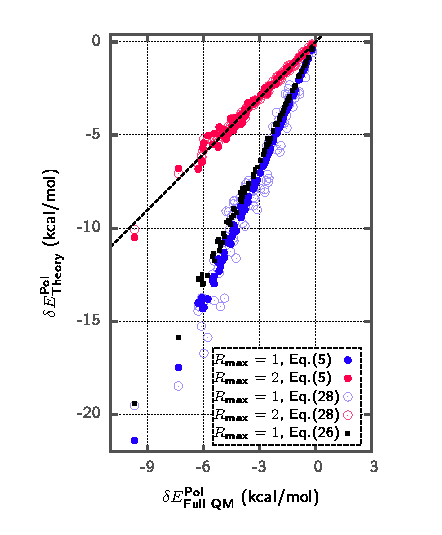
\includegraphics[width=0.5\textwidth]{data/dmatpol/water/figure1/fig-1.eps}
\caption{\label{f:fig-1} {\bf Performance of the DMS tensors of water molecule
in uniform electric field.} 
$R_{\rm max}$ denotes the maximum rank of the electric field
in the expansion from Eq.~\eqref{e:final-model.General}.
Electric field magnitudes in a range from 0.0 to 0.07 a.u. were tested in 100 samples with randomly selected 
directions of electric field.
} 
\end{figure}
%

All the tested models that are linear with respect to the electric field,
i.e., from Eq.~\eqref{e:final-model.HF} (black solid squares in Figure~\ref{f:fig-1}) 
as well as truncated at linear susceptibilities ${\bf B}^{(1)}$ 
from Eqs.~\eqref{e:dD-Taylor} (blue solid circles) and \eqref{e:final-model.General} (blue open circles),
incorrectly reproduce the polarization energy.
Interestingly, the predicted values are in strong
correlation with the exact estimates and exhibit a similar slope of $\sim$2.
Incorporation of the second\hyp{}order term
obtained either by numerical differentiation from Eq.~\eqref{e:B20} (red filled circles) 
or by using the generalized DMS model (red open circles)
dramatically reduces the errors
leading to quantitative accuracy in all tested field magnitudes 
with the best RMSE of 0.173 kcal/mol ($R^2=99.1\%$) for the generalized DMS model.
On the other hand, the
induced dipole and quadrupole moments are reproduced reasonably well by
using the first\hyp{}order DMS with $R^2$ coefficients being 
greater than 97\% in case of dipole moments and from 69\% up to 81\% in case of quadrupole moments.
This observation can be understood by the fact that the induced dipole
and quadrupole moment is approximately proportional to the external electric field, whereas the polarization
energy exhibits quadratic dependence (c.f. Eq.~\eqref{e:dE-dpol}), hence the need of including at least
quadratic terms in the expansion from Eq.~\eqref{e:dD-Taylor} or Eq.~\eqref{e:final-model.General}. 

In comparison to the dipole\hyp{}dipole polarizability approach, 
quadratic DMS models perform only slightly worse 
(for example, RMSE = 0.173 and 0.112 kcal/mol when the generalized quadratic DMS
model and the polarizability model are used, respectively).
However, quadratic DMS models better predict the induced multipole moments with
%work better
%when predicting the induced multipole moments with
$R^2$ systematically greater than 99\%. 
Certainly, taking into account the distributed quadrupole polarizabilities
would greatly reduce errors of the standard distributed polarizability approach.
Nevertheless, it is clear that the second\hyp{}order
DMS models are quantitative even at very strong uniform electric fields up to 0.07 a.u.
%On the other hand, DMS models better predict the induced dipole and quadrupole 
%moments even in weak fields. 

%
\begin{table*}%[]
\caption{{\bf Performance of the DMS tensors of water molecule
in uniform and non\hyp{}uniform electric field$^{a,b}$}
}
\label{t:results}
\begin{ruledtabular}
\resizebox{\textwidth}{!}{%
\begin{tabular}{cddddddcddddcdd}
%\hline\hline
\toprule
\multicolumn{1}{l}{} & \multicolumn{6}{c}{\textbf{Ab Initio DMS}} &  & \multicolumn{4}{c}{\textbf{Generalized DMS}}
                                                                  &  & \multicolumn{2}{c}{\textbf{Distributed}} \\
\cline{2-8}
\cline{9-12}
%\cline{14-15}
\textbf{}         
& \multicolumn{2}{c}{$\BM{R_{\rm max}=1}$$^c$}
& \multicolumn{2}{c}{$\BM{R_{\rm max}=1}$$^d$}
& \multicolumn{2}{c}{$\BM{R_{\rm max}=2}$$^d$}
&
& \multicolumn{2}{c}{$\BM{R_{\rm max}=1}$$^e$} 
& \multicolumn{2}{c}{$\BM{R_{\rm max}=2}$$^e$} 
&  
& \multicolumn{2}{c}{\textbf{Polarizability}}        \\ \hline
\multicolumn{15}{c}{} \\ 
\multicolumn{15}{c}{\textbf{Uniform Electric Field}} \\ 
\multicolumn{15}{c}{} \\ \hline
\multicolumn{1}{l}{} & \multicolumn{14}{c}{\textbf{RMSE (kcal/mol)}}              \\ %\hline
   & 4.041 & (n.d) & 4.823 & (n.d.) & 0.231 & (98.40) && 5.0121 & (n.d.) & 0.173 & (99.10) && 0.112 & (99.63) \\ 
\multicolumn{1}{l}{} & \multicolumn{14}{c}{\textbf{RMSD (mD)}}                    \\ %\hline
   & 30.46 & (97.91) & 30.46 & (97.91) & 18.02 & (99.27) && 24.83 & (98.61) & 7.13 & (99.89) && 30.46 & (97.91) \\ 
\multicolumn{1}{l}{} & \multicolumn{14}{c}{\textbf{RMSQ (D\AA $\times 10^{-3}$)}} \\ %\hline
   & 47.89 & (69.17) & 39.24 & (79.30) &  8.56 & (99.02) && 37.63 & (80.96) & 3.94 & (99.79) && 50.66 & (65.49) \\ \hline
\multicolumn{15}{c}{} \\ 
\multicolumn{15}{c}{\textbf{Non-Uniform Electric Field}$^{f}$} \\ 
\multicolumn{15}{c}{} \\ \hline
\multicolumn{1}{l}{} & \multicolumn{14}{c}{\textbf{RMSE (kcal/mol)}}   \\ 
W & 0.067 & (n.d.)     & - & (-) & - & (-) && 0.076 & (-)     & 0.003 & (99.45) && 0.004 & (98.64)\\ 
M & 1.072 & (n.d.)     & - & (-) & - & (-) && 1.236 & (-)     & 0.057 & (99.08) && 0.070 & (98.58)\\ 
S & 4.220 & (n.d.)     & - & (-) & - & (-) && 5.147 & (-)     & 0.402 & (97.25) && 0.332 & (98.13) \\ \hline
\multicolumn{1}{l}{} & \multicolumn{14}{c}{\textbf{RMSD (mD)}}  \\ 
W &  3.36 & (98.71) & - & (-) & -  & (-) &&  1.03 & (99.88) &  0.94 & (99.90) &&  3.36 & (98.71) \\ 
M & 14.72 & (98.50) & - & (-) & -  & (-) &&  7.72 & (99.59) &  4.55 & (99.86) && 14.72 & (98.50)\\ 
S & 44.80 & (96.92) & - & (-) & -  & (-) && 33.06 & (98.33) & 15.96 & (99.61) && 44.80 & (96.92) \\ \hline
\multicolumn{1}{l}{} & \multicolumn{14}{c}{\textbf{RMSQ (D\AA $\times 10^{-3}$)}} \\ 
W &  6.22 & (58.72) & - & (-) & - & (-) &&  1.59 & (97.32) &  1.42 & (97.86) &&  5.45 & (68.29) \\ 
M & 28.22 & (53.90) & - & (-) & - & (-) && 10.45 & (93.68) &  5.68 & (98.13) && 23.94 & (66.83) \\ 
S & 78.07 & (40.53) & - & (-) & - & (-) && 43.33 & (81.68) & 14.40 & (97.98) && 64.33 & (59.62) \\ 
\bottomrule
\end{tabular}%
}
\end{ruledtabular}
%
\footnotesize{\flushleft{
$^a$ $R$-squared coefficients are shown in parentheses. `$n.d.$' stands for `not determined'. 
$^b$ Ranks of the density matrix susceptibility models are denoted as $R_{\rm max}$ 
where $R_{\rm max}$ is the maximum power in the expansion from Eq.~\eqref{e:final-model.General}.
$^c$ \emph{Ab initio} HF model, Eq.~\eqref{e:final-model.HF}.
$^d$ \emph{Ab initio} finite\hyp{}difference model, Eq.~\eqref{e:dD-Taylor}.
$^e$ Linear\hyp{}regression generalized model, Eq.~\eqref{e:final-model.General}.
$^f$ `W', `M' and `S' denote `weak', `moderate' and `strong' electric fields 
that are generated by sets of point charges, respectively (c.f. Table~\ref{t:fields}).\\
}}
\end{table*}

\subsection{\label{ss:42}Water molecule in spatially non\hyp{}uniform electric field}

To study the capability of the distributed DMS models to capture 
density matrix polarization in inhomogeneous electric fields, we analyse a water molecule
surrounded by point charges.
Three different types of point charge environment that generate
weak (0.003 -- 0.007 a.u.), 
moderate (0.01 -- 0.02 a.u.) and strong (0.02 -- 0.05 a.u.) 
electric fields around the water molecule were considered (Table~\ref{t:fields}),
%
\begin{table}[b]
\caption{{\bf Average electric fields in statistical sets of electrostatically perturbed states
of water molecule surrounded by point charges$^a$}
}
\label{t:fields}
\begin{ruledtabular}
\begin{tabular}{ldcdcdcd}
\multirow{2}{*}{\textbf{Set$^b$}} & \multicolumn{7}{c}{\textbf{Average Electric Field (a.u.)}}      \\
                                  & \multicolumn{3}{c}{\textbf{Oxygen Atom}} & \textbf{} 
                                  & \multicolumn{3}{c}{\textbf{Hydrogen Atom}} \\
\cline{2-4}
\cline{6-8}
\textbf{W}                    & 0.0046     & $\pm$     & 0.0019     &           & 0.0046     & $\pm$     & 0.0020     \\
\textbf{M}                    & 0.0184     & $\pm$     & 0.0075     &           & 0.0186     & $\pm$     & 0.0078     \\
\textbf{S}                    & 0.0368     & $\pm$     & 0.0150     &           & 0.0372     & $\pm$     & 0.0156    
\end{tabular}
\end{ruledtabular}
%
\footnotesize{\flushleft{
$^a$ Each set was composed of 100 samples differing in the configuration of 40 charges generated from a uniform distribution.
$^b$ `W', `M' and `S' denote `weak', `moderate' and `strong' electric fields, respectively.\\
}}

\end{table}
%
because similar ranges of electric field are experienced by water molecules
in liquid phase.\cite{Reischl.Kofinger.Dellago.MolPhys.2009,Fried.Wang.Boxer.Ren.Pande.JPCB.2013}
Performance descriptors of the \emph{ab initio} and generalized 
models of the density matrix susceptibility, as well as 
the conventional dipole\hyp{}dipole distributed polarizability
approach, are shown in Table~\ref{t:results}. 

Similarly as in uniform electric field, 
the \emph{ab initio} DMS model from Eq.~\eqref{e:final-model.HF} 
as well as
the linear generalized DMS model, are insufficient to correctly describe the polarization energy 
in non\hyp{}uniform electric field,
although the correlation with benchmark is still very clear with a slope of $\sim$2
(Figure~\ref{f:fig-2}A). 
Again, induced dipole moments are reproduced very well even
in strong electric fields (RMSD of 44.8~mD and lesser, $R^2>96\%$).
Induced quadrupole moments are well described only by the generalized DMS model.
For example, in medium electric fields RMSQ is 10.4$\times 10^{-3}$D\AA{ }with $R^2=93.7\%$
whereas the \emph{ab initio} DMS model yealds RMSQ of 28.2$\times 10^{-3}$D\AA{ }($R^2=53.9\%$).

The most sophisticated model studied in this work, the generalized quadratic DMS model, yields excellent predictions 
of the polarization energies and induced multipole moments in all strengths of the non\hyp{}uniform electric field tested.
The errors in predicting polarization energy are reduced by an order of magnitude when compared with
the linear DMS models. Improvement of accuracy can also be observed in the case of induced multipole moment predictions
but the effect is less significant (improvement roughly by a factor of 2).
What is particularly interesting is that in weak and moderate electric fields
the generalized quadratic DMS model performs better than the distributed dipole\hyp{}dipole
polarizability model, whereas only in strong electric fields the situation is reversed
(RMSE of 0.402, $R^2=97.2\%$ and 0.332 kcal/mol, $R^2=98.2\%$ for the DMS and polarizability model, respectively).
Nevertheless, the quadratic DMS model yields still very high $R^2$ of 97.2\% even in strong electric fields for polarization
energy, and also very high $R^2$ for induced multipole moments.

Recently, it was found by Fried et~al. by performing molecular dynamics simulations with a classical 
polarizable force field, that the average electric field experienced by water molecule in liquid phase
in room temperature is around 0.014 a.u. ($\sim$70 MV/cm).\cite{Fried.Wang.Boxer.Ren.Pande.JPCB.2013}
This value corresponds to our moderate electric field set of samples (denoted as `M' in Tables~\ref{t:results}
and \ref{t:fields}) for which the
accuracy of the generalized quadratic DMS model is excellent.
Water molecules can experience
stronger electric fields in certain geometries of hydrogen bonded clusters, 
even up to 0.055 a.u. according to study by Reischl et~al.\cite{Reischl.Kofinger.Dellago.MolPhys.2009} 
This electric field magnitude falls into our strong electric field regime (denoted as `S')
in which the generalized quadratic
DMS model still provides accurate predictions (see also error distributions 
shown in Figure~\ref{f:fig-2}B, \ref{f:fig-2}E and \ref{f:fig-2}H). 
Even at the current state of development, the generalized DMS model
is of comparable energetic accuracy as the distributed polarizability model. 
It is emphasized here that the model can be extended by taking into account
third\hyp{}order terms which should reduce the errors even further.
%This however falls out of scope of this contribution and it will be studied
%elsewhere. 
Therefore, it is believed that
the generalized DMS approach
has an important advantage over the multipole\hyp{}based approach, i.e., it provides detailed
tensor description of the spatial polarization of the electron density distribution, that could be
combined with density\hyp{}based methods of interaction energy calculations.\cite{Mandado.Hermida-Ramon.JCTC.2011}

\begin{figure*}[h]
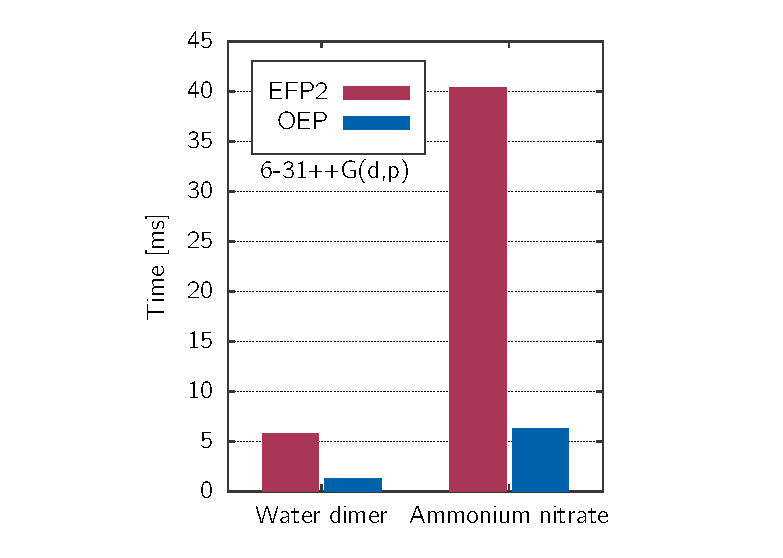
\includegraphics[width=\textwidth]{data/dmatpol/water/figure1/fig-2.eps}
\caption{\label{f:fig-2} {\bf Performance of the distributed DMS tensors of water molecule in moderate
non\hyp{}uniform electric fields.}
In this Figure, `Ab Initio DMS' (panels A, D and G) 
refers to the model from Eq.~\eqref{e:final-model.HF} and
`Generalized DMS' (panels B, E and H) 
refers to the generalized model with $R_{\rm max}=2$ 
where $R_{\rm max}$ is the maximum power
in the expansion from Eq.~\eqref{e:final-model.General}.
%Calculations of the electric field\hyp{}induced interaction energies (A-C), dipole moments (D-F) and
%quadrupole moments (G-I). 
Comparison with the distributed dipole\hyp{}dipole polarizability model 
is also shown in this Figure in panels C, F and I.}
\end{figure*}

\section{\label{s:5}Summary and a few concluding remarks}

In this work, the \emph{ab initio} model of the one\hyp{}particle density matrix susceptibility tensors
at the HF level was derived for a closed shell molecule in a spatial
electric field distribution. It was found that the change in the density matrix element
is approximately linearly proportional to the electric field evaluated at the distributed site associated with the 
center of charge of the 
localized molecular orbital. Subsequently, the \emph{ab initio} model served as a basis
for the formulation of the generalized model that is, in principle, not limited to the HF theory,
and takes into account also quadratic and higher\hyp{}order terms with respect to the electric field.
The generalized model, which consisted of a set of adjustable parameters,
definined the first\hyp{} and second\hyp{}order density matrix susceptibilities
that were determined through the least\hyp{}squares 
linear regression with respect to the training ensemble of electrostatically perturbed states.

The above theoretically developed models were then used to calculate the electric field\hyp{}induced
interaction energies, dipole moments and quadrupole moments of water molecule that
interacts with uniform electric fields as well as 
various point charge environments generating electric fields of weak, moderate
and strong magnitudes. It was found that, while the \emph{ab initio} model yields qualitatively incorrect
interaction energies, the generalized model can reach quantitative level of accuracy
for prediction of interaction energies, dipole moments and even quadrupole moments
once, at least quadratic terms with respect to the electric field, are taken into account. 
This work demonstrated that it is possible to
accurately predict the change in the density matrix of electronic system, and the accuracy of the model
can be improved by extending the parameter space of the susceptibility tensors. 

It is anticipated here that the generalized models from Eq.~\eqref{e:final-model.General}
should be studied in the future with an emphasis 
on their further optimization.
%, especially to reach RMSE below 1 kcal/mole
%in strong and very strong electric fields (0.05-0.07 a.u.). 
For this purpose, more general forms of Eq.~\eqref{e:final-model.General}, as well as the choice of distributed
sites should be further investigated, preferably with post\hyp{}Hartree\hyp{}Fock methods
and electronically excited states.
Nevertheless, owing to the capability of the proposed approach to correctly capture the 
environment\hyp{}induced changes in the one\hyp{}particle density matrix, 
the generalized density matrix susceptibility tensors 
could be used in accurate fragment\hyp{}based calculations of extended molecular aggregates
described at correlated levels of theory, particularly including the excited state chemistry.

\begin{acknowledgments}
This project is carried out under POLONEZ programme which has received funding from the European Union's
Horizon~2020 research and innovation programme under the Marie Skłodowska-Curie grant agreement 
No.~665778. This project is funded by National Science Centre, Poland 
(grant~no. 2016/23/P/ST4/01720) within the POLONEZ 3 fellowship.
%Many thanks to Robert W.~G{\'o}ra and Robert Zale{\'s}ny 
%for reading and commenting on the manuscript.
\end{acknowledgments}

%
\appendix

\section{\label{a:orig-dep} Origin-Independence of the Induced Dipole Moment}

Multipole integrals depend on the origin with respect to which they are evaluated.
However, the induced dipole moments defined in Eq.~\eqref{e:dmu-4-exact.linear-approximation} 
(or equivalently in Eq.~\eqref{e:dmu-l-vector})
have to be origin independent. Note that
%
\begin{equation}
 \left[ \widetilde{\mathbb{M}} \right]_{i\alpha} ({\bf r}_Q) 
 = \left[ \widetilde{\mathbb{M}} \right]_{i\alpha} ({\bf 0}) - \left[ {\bf C}^\dagger \right]_{i\alpha} {\bf r}_Q  
\end{equation}
%
and
%
\begin{equation}
 \left[ \widetilde{\mathbb{K}} \right]_{i\alpha} ({\bf r}_Q) 
 = \left[ \widetilde{\mathbb{K}} \right]_{i\alpha} ({\bf 0}) - \left[ {\bf C}^\dagger \cdot {\bf D} \right]_{i\alpha} {\bf r}_Q \;.
\end{equation}
%
But ${\bf C}^\dagger \cdot {\bf D}={\bf C}^\dagger \cdot {\bf C} \cdot {\bf C}^\dagger={\bf C}^\dagger$ in orthogonal
AO basis which implies that
%
\begin{multline}
   \left[ \widetilde{\mathbb{L}} \right]_{i\alpha} ({\bf r}_Q) 
 = \left[ \widetilde{\mathbb{M}} \right]_{i\alpha} ({\bf r}_Q) 
 - \left[ \widetilde{\mathbb{K}} \right]_{i\alpha} ({\bf r}_Q) \\
 = \left[ \widetilde{\mathbb{M}} \right]_{i\alpha} ({\bf 0})   
 - \left[ \widetilde{\mathbb{K}} \right]_{i\alpha} ({\bf 0})
 = \left[ \widetilde{\mathbb{L}} \right]_{i\alpha} ({\bf 0}) \;.
\end{multline}
%
Therefore, it is proved that the polarization\hyp{}induced distributed dipole moments 
defined in Eq.~\eqref{e:dmu-4-exact.linear-approximation} are origin independent.
Thus, one can compute dipole integrals with respect to any origin and resulting
susceptibilities ${\bf B}_{\alpha\beta}^{(i;1)}$ from Eq.~\eqref{e:susceptibility-B} will be uniquely defined.

\section{\label{a:blocks} Explicit Formulae for Gradient and Hessian Blocks in Linear Regression DMS Model}

The gradient vector ${\bf g}$ and Hessian matrix ${\bf H}$ 
are build from blocks associated with a particular type of parameters, i.e.,
%
\begin{equation}\label{e:Newton.gH}
 {\bf g} = 
\begin{pmatrix}
{\bf g}^{[1]} \\ 
{\bf g}^{[2]} 
\end{pmatrix} ,\quad
 {\bf H} = 
\begin{pmatrix}
{\bf H}^{[11]} & {\bf H}^{[12]}  \\ 
{\bf H}^{[21]} & {\bf H}^{[22]}  
\end{pmatrix} \;,
\end{equation}
%
where the block indices 1 and 2 correspond to the first\hyp{} and second\hyp{}order susceptibilities, respectively.
Note that the second derivatives of $\delta D^{(N)}$ 
with respect to the adjustable parameters vanish
due to the linear functional form of Eq.~\eqref{e:final-model.General.Parameters}.
Thus, the gradient element of the $r$th block and Hessian element of the $(rs)$th block read
%
\begin{subequations}
 \begin{align}
  g^{[r ]}    &\equiv \frac{\partial   Z}{\partial S^{[r]}} 
     =-2\sum_N \overline{\delta D}^{(N)}
               \frac{\partial   \left[ \delta D^{(N)} \right]}{\partial S^{[r]}} \;,\\
  H^{[rs]} &\equiv \frac{\partial^2 Z}{\partial S^{[r]} \partial S^{[s]}}  
     = 2\sum_N 
        \frac{\partial   \left[ \delta D^{(N)} \right]}{\partial S^{[r]}}
        \frac{\partial   \left[ \delta D^{(N)} \right]}{\partial S^{[s]}} \;.
 \end{align}
\end{subequations}
%
The explicit formulae for the gradient are
%
\begin{subequations}
 \begin{align}
  g^{[1]}_{ku} &=-2\sum_N \overline{\delta D}^{(N)} F^{(N)}_{ku} \;,\\
  g^{[2]}_{kuw} &=-2r_{uw} \sum_N \overline{\delta D}^{(N)} F^{(N)}_{ku} F^{(N)}_{kw} \;.
 \end{align}
\end{subequations}
%
The Hessian subsequently follows to be
%
\begin{subequations}
 \begin{align}
  H^{[11]}_{ku,lw} &= 2\sum_N F^{(N)}_{ku} F^{(N)}_{lw} \;,\\
  H^{[12]}_{ku,lu'w'} &= 2r_{u'w'} \sum_N F^{(N)}_{ku} F^{(N)}_{lu'} F^{(N)}_{lw'}  \;,\\
  H^{[22]}_{kuw,lu'w'} &= 2r_{uw} r_{u'w'} \sum_N F^{(N)}_{ku} F^{(N)}_{kw} F^{(N)}_{lu'} F^{(N)}_{lw'} \;.
 \end{align}
\end{subequations}
%
Note that due to the symmetry of the Hessian matrix, the block $21$
is a transpose of the block $12$. 
The composite indices $ku$ and $kuw$ are constructed from the distributed site index $k$
and the appropriate symmetry\hyp{}adapted ($w<u$) Cartesian component 
of a particular DMS tensor: $u$ for the first\hyp{}order,
and $uw$ for the second\hyp{}order susceptibility tensor, respectively.

% -----------------------
\bibliography{references}
% -----------------------

\end{document}
